\documentclass{standalone}
\usepackage{tikz}
\usetikzlibrary{arrows.meta, decorations.markings, intersections, positioning}

\begin{document}
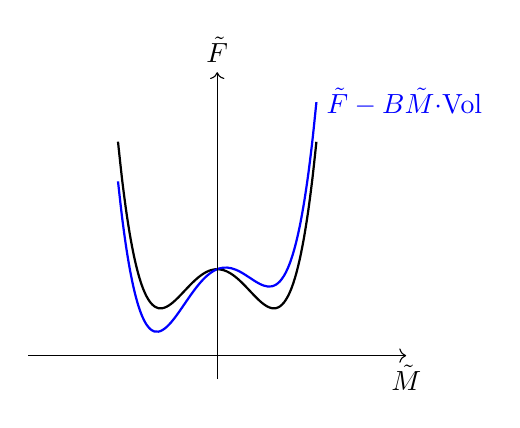
\begin{tikzpicture}[scale=.6]
\def\a{1.2}
\def\b{.4}



% \draw[gray, very thin, step=1] (-3.9,-.9) grid[] (3.9,3.9);

\draw[thick] plot[smooth, samples=50, domain=-2.1:2.1] (\x, {\b * (\x*\x - \a*\a)*(\x*\x - \a*\a)});

\draw[thick, blue] plot[smooth, samples=50, domain=-2.1:2.1] (\x, {.4 * \x + \b * (\x*\x - \a*\a)*(\x*\x - \a*\a)})
node [right,blue]{$\tilde{F} - B \tilde{M}\cdot$Vol};

\draw[ -> ] (-4,-1) -- (4,-1) node[below] {$\tilde{M}$};
\draw[ -> ] (0,-1.5) -- (0,5) node[above] {$\tilde{F}$};


\end{tikzpicture}
\end{document}